\chapter{Design and Implementation}\label{chap:design-implementation}


\section{System Architecture Overview (PC--Android System Design)}\label{sec:4-1}
The system employs a client-server architecture with a central PC coordinating multiple Android capture devices (see ADR-001: Reactive State Management for the rationale). The PC application acts as the master controller, connecting to each Android device over a local network. Each Android device runs a capture app that records sensor data and video, while the PC offers a unified interface to start/stop recordings and aggregate data.

The system architecture (see Figure~\ref{fig:4_01_arch_overview} in Appendix I) shows how the PC communicates with Android smartphones via Wi-Fi using a custom TCP/IP protocol, sending commands and receiving telemetry (video previews, sensor readings). Android devices autonomously capture data with high-precision clocks for local timestamps, synchronised to the PC's timeline through network time alignment. This design enables multiple phones to record simultaneously within a single session, with the PC serving as the time base. The PC can also integrate local hardware (e.g., a webcam and GSR sensor) alongside the Android data. All captured modalities (video streams, audio, thermal data, GSR signals) are temporally aligned and consolidated on the PC. The result is a distributed recording system where diverse data sources function as a single synchronised unit.


\section{Android Application Design and Sensor Integration}\label{sec:4-2}
The Android application is designed for coordinated multi-modal data capture. At its core is a \texttt{RecordingController} class managing all hardware components and recording tasks. This controller prepares subsystems -- cameras (RGB and thermal), physiological sensors (GSR/PPG), a microphone, etc. When a recording session begins, the controller initialises a new session directory and starts all enabled sensor/camera captures with nanosecond-precision timestamps. Each modality's data is written to device storage in real time. The design utilizes modern Android libraries for performance: CameraX for efficient video and image capture \cite{ref13} and the Nordic BLE library for reliable Bluetooth Low Energy communication with sensors \cite{ref14}. All sensor readings and frames are timestamped with a monotonic clock source to ensure consistency. This modular design (ADR-003: Function Decomposition Strategy) allows easy enabling/disabling of features based on device capabilities (e.g., an inactive thermal camera module if not attached). It also simplifies synchronisation, enabling the controller to manage data sources uniformly (start all, stop all) and trust their timestamps. This modular approach (following ADR-003: Function Decomposition Strategy) facilitates easy feature management based on device capabilities (e.g., inactive thermal camera module). It also streamlines synchronisation logic, enabling uniform handling of data sources (start all, stop all) and reliable timestamping of outputs.

The Android app's internal architecture for thermal camera integration is detailed in Figure~4.2 (see Appendix I), which provides an overview of the data flow and component interactions.

The following subsections detail the integration of the Topdon thermal camera and Shimmer GSR sensor in the Android app.

\subsection{Thermal Camera Integration (Topdon)}\label{sec:4-2-1}
Integrating the Topdon TC001 thermal camera on Android required using USB host mode and a UVC (USB Video Class) library. The app utilises the open-source Serenegiant USB Camera library (UVCCamera) for USB Video Class device support \cite{ref16} to interface with the device. A dedicated class \texttt{TopdonThermalCamera} implements the \texttt{ThermalCamera} interface and encapsulates all thermal camera functionality. When the camera is physically connected via USB-C, an Android USB monitor detects the device. The \texttt{TopdonThermalCamera} registers a \texttt{USBMonitor.OnDeviceConnectListener} to handle attachment events. On a successful connection, it opens the UVC device and configures it to the desired frame size and mode before starting the video stream \cite{ref16}. By default, the camera is set to its native thermal resolution (256\,\texttimes\,192 pixels) and begins previewing immediately on a background thread.

The library provides a framebuffer in \texttt{ByteBuffer} format for each incoming thermal frame. The implementation registers a frame callback to retrieve this data stream. In the callback, the code reads raw temperature data as an array of 16-bit (or 32-bit) values, then writes each frame's timestamp and temperature data to a CSV file. Each row represents a frame, starting with a high-resolution timestamp (in nanoseconds), followed by the temperature values of all 49{,}152 pixels (256\,\texttimes\,192) in that frame \cite{ref16}. This logging creates a large but detailed dataset, effectively a thermal video as numeric data per frame. To maintain performance, the thermal capture runs in its own thread context (within the UVCCamera library's callback) preventing disk writing from blocking the main UI or other sensors. Heavy processing is avoided during capture, using a Lab Streaming Layer (LSL) marker for event marking (synchronisation or debugging) via an LSL marker \cite{ref9}.

The thermal camera logging implementation is in Appendix F.1 (see Listing F.1 for the complete code).

The Topdon camera operates over USB, with the app managing permissions and device registration. The \texttt{TopdonThermalCamera} calls \texttt{usbMonitor.register()} at startup to listen for devices \cite{ref16} and unregisters on pause to free resources. If the device is detected, the user is prompted to grant access. Once granted, the \texttt{TopdonThermalCamera.open()} method uses the USB monitor to obtain a control block and create a \texttt{UVCCamera} instance \cite{ref16}. The camera is configured and marked as connected. If a preview surface is available, it can be attached via \texttt{startPreview(surface)} to render the thermal feed live \cite{ref16}. Previewing is optional; frames are captured and logged regardless. To stop the thermal camera, the preview (if any) is halted, the frame callback is disabled, the file writer is closed, and the UVC camera instance \cite{ref16}. This orderly shutdown ensures the USB device is available for future sessions. The Topdon integration captures thermal frames at 256\,\texttimes\,192 resolution, with each frame containing 49{,}152 temperature values in CSV format. Frame capture occurs at regular intervals, validated by the UVCCamera library's callback mechanism for precise alignment with RGB video and physiological signals.

\subsection{GSR Sensor Integration (Shimmer)}\label{sec:4-2-2}
The Android app connects to a Shimmer3 GSR+ sensor to record Galvanic Skin Response (GSR) and photoplethysmography (PPG) data. It utilises Bluetooth Low Energy (BLE). The \texttt{ShimmerGsrSensor} class extends Nordic's BLE manager to handle the GSR sensor's protocol. The Shimmer employs UART-over-BLE: one characteristic (TX) sends commands while the other (RX) receives notifications. The app's \texttt{ShimmerGsrSensor} knows the byte commands for streaming control. Sending \texttt{0x07} starts the live data stream, and \texttt{0x20} ends it \cite{ref15}. Sending \texttt{0x07} starts the live data stream, and \texttt{0x20} ends it \cite{ref15}.

When enabled, the \texttt{RecordingController} creates a \texttt{ShimmerGsrSensor} instance at startup. If GSR recording is enabled, the controller starts a recording session by invoking \texttt{physiologicalSensor.startStreaming(...)} with a file writer. This connects the BLE manager (if needed) and sends the Start Streaming command (\texttt{0x07}) to the sensor's TX characteristic \cite{ref15}. The Shimmer device sends notifications (about 128 Hz) on the RX characteristic, containing GSR and PPG readings. The \texttt{ShimmerGsrSensor} sets up a notification callback in its GATT callback's \texttt{initialise ()} method to handle incoming packets \cite{ref15}. As data arrives, the \texttt{onShimmerDataReceived()} function parses the byte payload per Shimmer's data protocol \cite{ref8}. The first byte indicates a standard data packet (\texttt{0x00}), followed by sensor readings. Each 8-byte packet includes two bytes for PPG, two for GSR, and additional info. The app reconstructs the 16-bit raw PPG and GSR values from the byte sequence \cite{ref8}. The GSR reading includes a range indicator in the top bits, as Shimmer uses multiple gain ranges. The implementation extracts the range and applies the conversion formula to derive resistance, inverting it to obtain conductance in microsiemens. This follows Shimmer's conversion guidelines \cite{ref8}; for instance, a 40.2 k$\Omega$ resistor uses the formula $\mathrm{GSR}\ (\mu\mathrm{S}) = \frac{1}{R} \times 1000$, with $R$ computed from the 14-bit ADC value. Similar formulas apply to other ranges (287 k$\Omega$, 1 M$\Omega$, 3.3 M$\Omega$) \cite{ref8}. Each data point includes a timestamp, a GSR value (in $\mu$S), and a raw PPG value after conversion.

Every GSR/PPG sample is written to a CSV file by the app. The \texttt{ShimmerGsrSensor} maintains a file writer stream; it writes a header line (\texttt{timestamp\_ns, GSR\_uS, PPG\_raw}) and appends each new sample. The timestamp is obtained via the app's \texttt{TimeManager.getCurrentTimestampNanos()} for consistency with other modalities. The app also streams live data for video synchronisation; the \texttt{RecordingController} provides a callback to \texttt{startStreaming()}, pushing each sample into a local Lab Streaming Layer (LSL) outlet named \texttt{"Android\_GSR"} \cite{ref9}. This allows real-time monitoring of GSR data without burdening the UI thread. Streaming and logging occur in a background thread, ensuring notifications do not block the UI. If the BLE connection drops or has an error, the Nordic library's retry mechanism attempts reconnection up to 3 times with a short delay \cite{ref14}. The app also ensures graceful shutdown: when recording stops, it sends the stop command (\texttt{0x20}) to halt streaming \cite{ref15} and closes the file writer. This ensures proper finalisation of the CSV.

The complete Shimmer GSR sensor BLE streaming and logging implementation is in Appendix F.2 (see Listing F.2 for the code).

\begin{figure}[htbp]
    \centring
    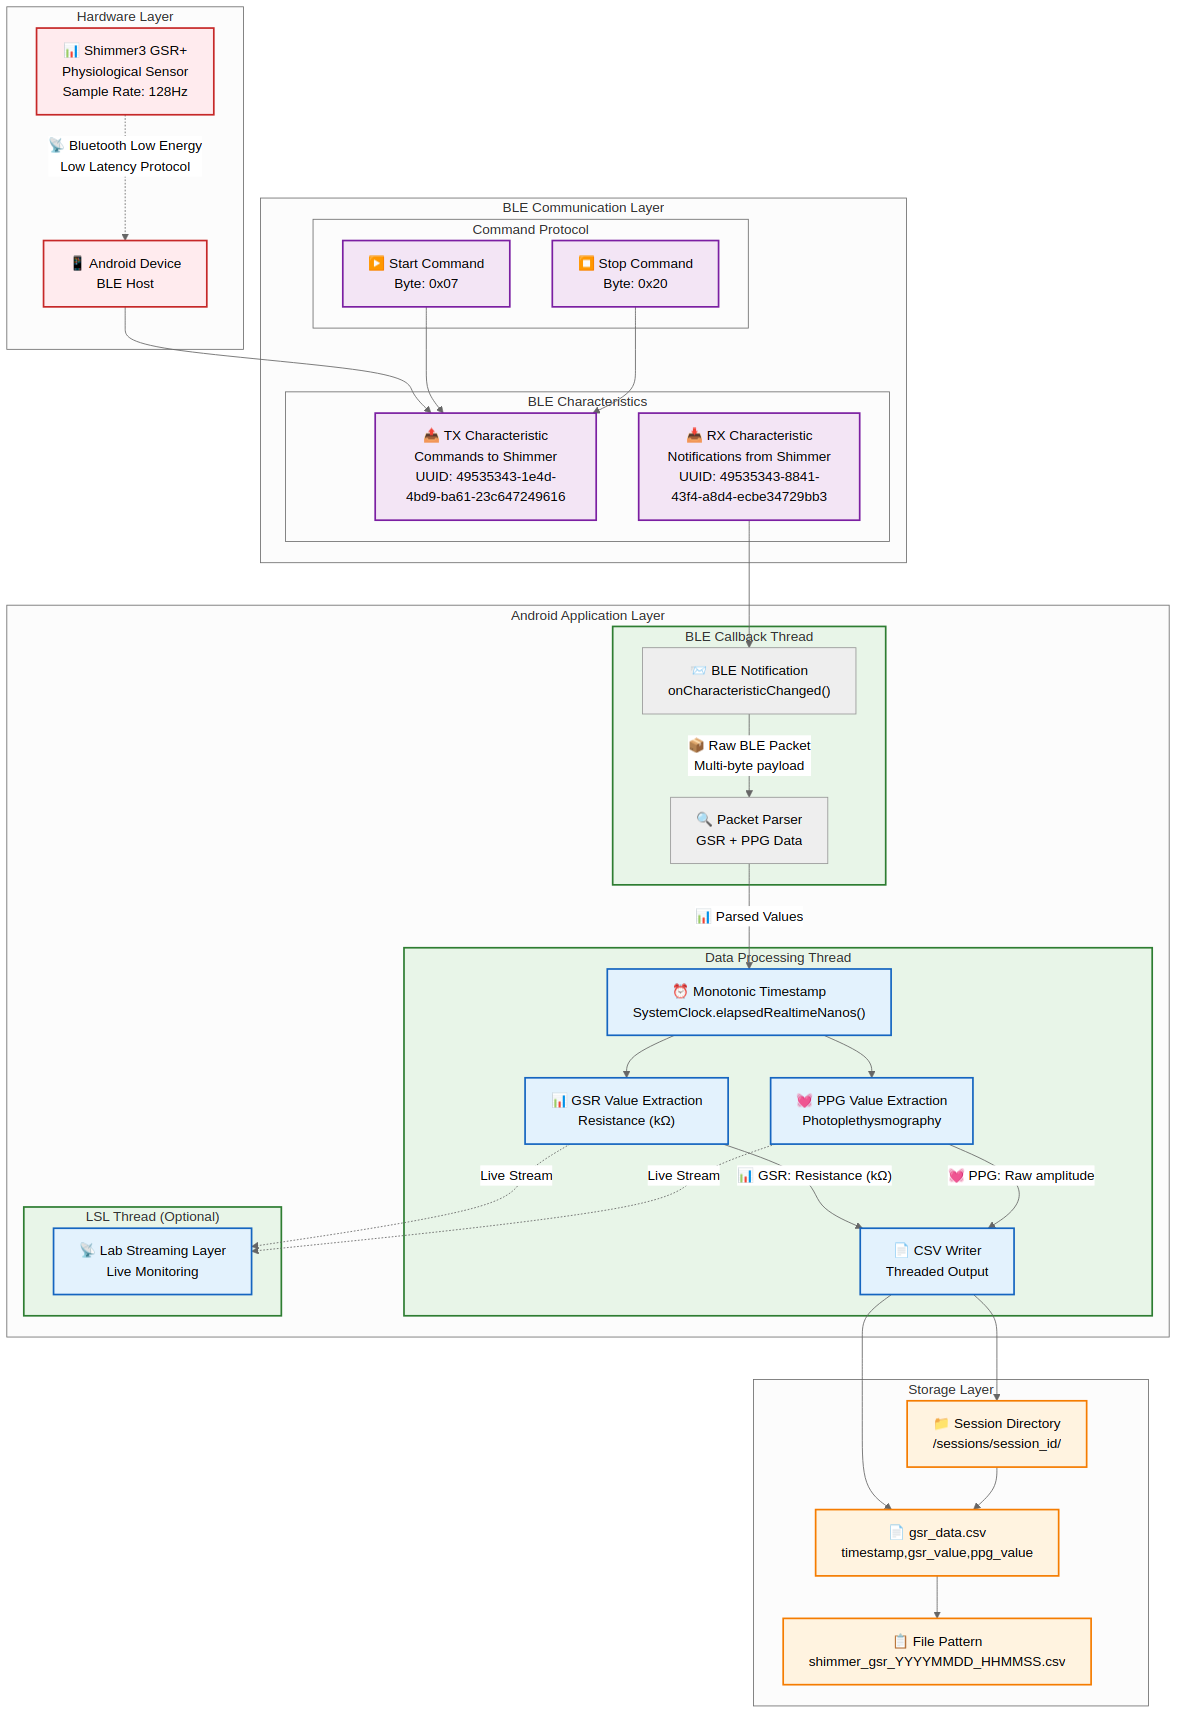
\includegraphics[width=\textwidth]{../diagrams/fig_4_03_shimmer_gsr_integration.png}
    \caption{Shimmer GSR Integration illustrating the desktop controller application architecture.}
    \label{fig:4_03_shimmer_gsr_integration}
\end{figure}

The Shimmer integration streams GSR/PPG data at a 128 Hz sampling rate with real-time conversion from raw ADC values to microsiemens using device-specific calibration formulas. Data is written simultaneously to CSV files and LSL streams, enabling both persistent storage and live monitoring with temporal synchronisation maintained through the \texttt{TimeManager.getCurrentTimestampNanos()} method.


\section{Desktop Controller Design and Functionality}\label{sec:4-3}
The desktop controller is a cross-platform application (tested on Windows, Linux, and macOS) built with Qt for the GUI (PyQt6/PySide6) \cite{ref17} and Python 3 for logic, augmented by performance-critical C++ components. The implementation initialises a main window with a tabbed interface. The Dashboard tab provides an overview of connected devices and local sensors, displaying live video feeds and GSR plots in a grid layout. The code sets up a \texttt{QLabel} for video preview and a PyQtGraph \texttt{PlotWidget} for GSR. For example, it can display live video feeds and GSR plots in a grid layout -- the code sets up a \texttt{QLabel} for a video preview and a PyQtGraph \texttt{PlotWidget} for GSR on the dashboard. A Logs tab captures real-time system messages (status updates, errors) for debugging. Another tab for Playback \& Annotation allows reviewing recorded sessions (in a later implementation phase). Each tab's UI elements are created and managed with Qt layouts, making the interface flexible and scalable as devices are added.

The PC controller uses background threads for networking and data processing, preventing UI freezes. A dedicated \texttt{WorkerThread} (a \texttt{QThread} subclass) is responsible for all communication with Android devices. When the user initiates a connection to a device, this worker thread opens a TCP socket to the phone's IP and port. The thread then runs an event loop, receiving JSON messages from the device. When an Android phone sends a preview frame update, the worker decodes the base64 image bytes to a \texttt{QImage} and emits a \texttt{newPreviewFrame} signal with the image and device ID. For instance, if a connected Android phone sends a preview frame update, the worker decodes the base64-encoded image bytes to a \texttt{QImage} and emits a \texttt{newPreviewFrame} signal carrying the image and device identifier. The main GUI thread connects this signal to a slot that displays the frame in the dashboard (e.g., updating the corresponding \texttt{QLabel}'s pixmap). The worker also handles command responses: every command sent to a device includes a unique ID, and the device's reply includes an \texttt{ack\_id} with status info. For example, a \texttt{"capabilities\_data"} response contains the list of cameras the device has -- the worker emits a \texttt{camerasReceived} signal with that list so the UI can populate camera options. This asynchronous message-passing design keeps the GUI responsive and enables the PC to manage multiple devices simultaneously by spawning separate threads for each connection.

The signal-slot mechanism for preview frames is implemented using PyQt's asynchronous messaging system, with details in Appendix F.3 (see Listing F.3 for complete code).

The application uses Zeroconf (mDNS) \cite{ref19} for device discovery: upon startup, the PC browses for \texttt{\_gsr-controller.\_tcp} services on the local network. Each Android device advertises this service type with a name like \texttt{"GSR Android Device [Model]"}. The PC automatically lists available devices and their corresponding addresses, eliminating the need for manual IP entry.

A key feature of the PC controller is its native C++ backend for time-sensitive hardware interaction. This is implemented as a Python extension module (via PyBind11) \cite{ref18} named \texttt{native\_backend}. It provides classes \texttt{NativeWebcam} and \texttt{NativeShimmer} that run in background threads to deliver data to Python with minimal latency. The controller instantiates these at startup: for example, \texttt{NativeWebcam(0)} opens the local webcam (device 0) and begins capturing frames in a loop, and \texttt{NativeShimmer("COM3")} connects to a Shimmer GSR device via a serial port (COM3 on Windows). These native objects start immediately and run independently of the Python GIL, pushing data into thread-safe queues. The GUI uses a \texttt{QTimer} tick (~16 ms) to retrieve the latest data periodically from the native threads. On each tick, it pulls a frame from the webcam class (as a NumPy array) and updates the corresponding video label \cite{ref1}, \cite{ref2}. Similarly, it polls the Shimmer class for new GSR samples and updates the live plot. The native backend captures at a steady ~60 FPS by sleeping ~16 ms per iteration, and yields frames without significant buffering. Meanwhile, the Shimmer thread reads sensor bytes as fast as they arrive (128 Hz) with precise timing. Both use lock-free queues to decouple production and consumption of data. The C++ code directly converts camera frames to a shared memory buffer that is exposed to Python as a NumPy array without copying \cite{ref1}, \cite{ref2}, and similarly packages GSR readings into Python tuples. This design minimises overhead, latency, and jitter -- imperative for synchronising local PC data with remote device data.

Beyond live monitoring, the desktop app includes tools for post-session analysis. The Playback \& Annotation tab (Figure~4.4) is designed to load the recorded video files (RGB and thermal) in a synchronised fashion. The controller employs OpenCV and pandas to process data along a unified timeline, displaying the video frame and corresponding GSR plot point at the selected timestamp. Users can add annotations at specific times, which can be saved in a sidecar file or embedded in session metadata. The PC software also features a Calibration utility for camera calibration post-recording. Using OpenCV \cite{ref22}, it detects calibration patterns (such as chessboards or ChArUco markers) in raw RGB frames to calculate the intrinsic camera parameters. If multiple cameras (e.g., a phone’s RGB and thermal, or a phone and PC webcam) observe the same pattern, it computes their extrinsic calibration. The results, like camera matrices, distortion coefficients, and transformation matrices are saved for data processing. The controller can also export data (often downsampled or compressed) into a single file per session for distribution or analysis. Thus, the desktop controller provides live data acquisition coordination and comprehensive post-processing tools, designed as a modular PyQt6 application with a tab-based architecture.

\begin{figure}[htbp]
    \centring
    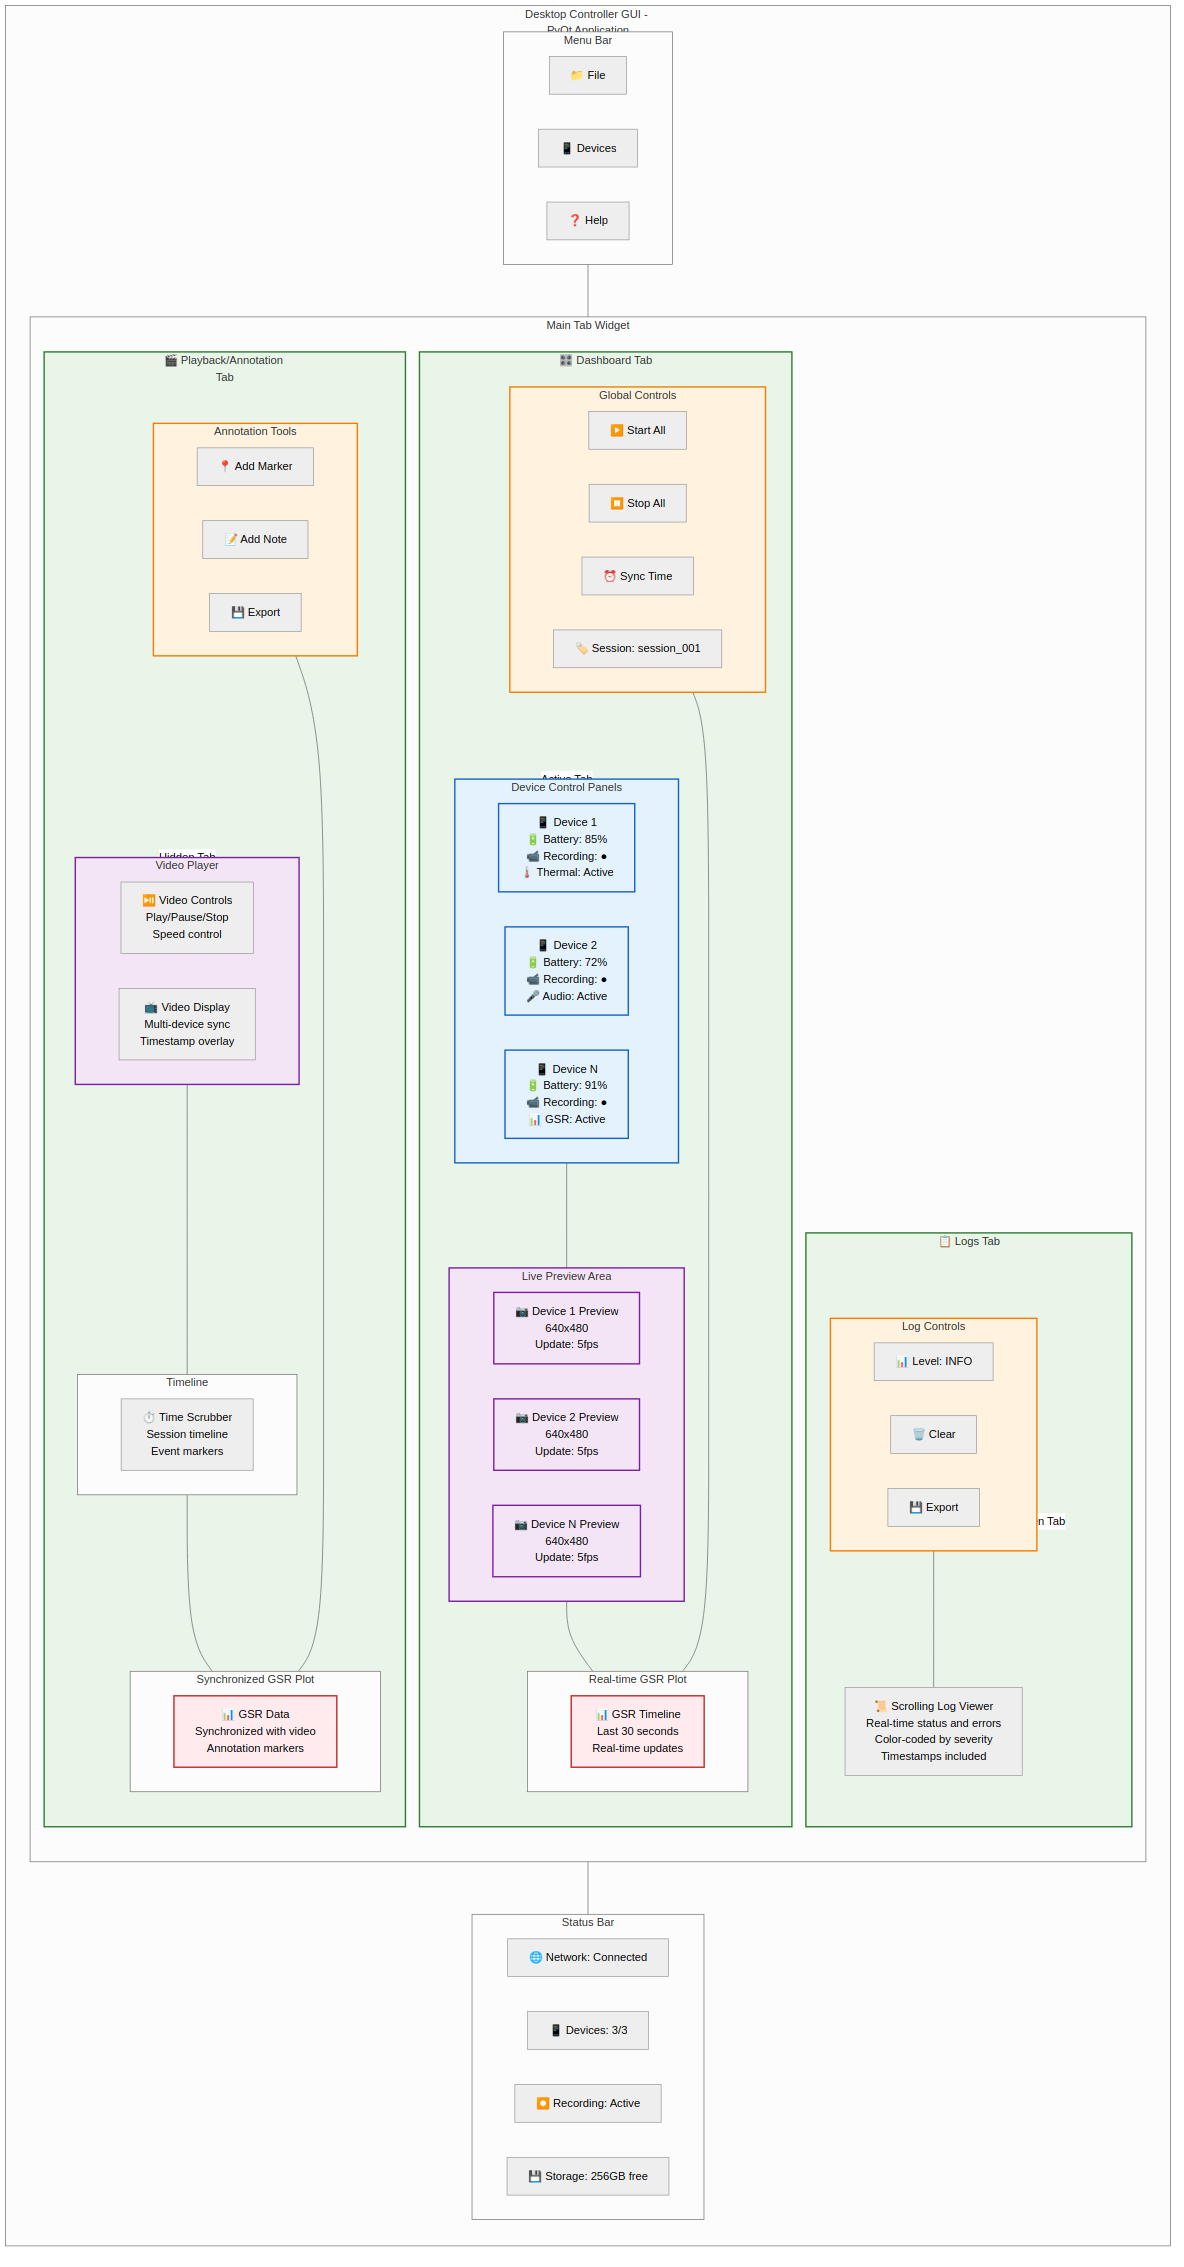
\includegraphics[width=\textwidth]{../diagrams/fig_4_04_desktop_gui_layout.png}
    \caption{Desktop GUI Layout illustrating the playback and annotation interface described above.}
    \label{fig:4_04_desktop_gui_layout}
\end{figure}


\section{Communication Protocol and Synchronisation Mechanism}\label{sec:4-4}
A custom communication protocol connects the PC controller with each Android device, built on TCP/IP sockets \cite{ref21} with JSON message payloads. After the PC discovers an Android device (via Zeroconf), it initiates a TCP connection to the device's advertised port. The Android app runs a lightweight TCP server to accept this connection. All commands from PC to Android are sent as JSON objects with a schema like \texttt{\{"id": <command\_id>, "command": "<action>", "params": \{ ... \}\}}. The device, upon receiving a command, executes the requested action and then replies with a JSON response containing the original command ID (as \texttt{ack\_id}) and a status or result. For example, the first command the PC sends is \texttt{"query\_capabilities"}, which asks the phone to report its hardware capabilities. The Android app responds with a message like \texttt{\{"ack\_id": 1, "status": "capabilities\_data", "capabilities": \{ ... \}\}} including details such as available cameras (with their identifiers, resolutions, and frame rates). This exchange allows the PC to dynamically adjust to each device -- for instance, listing the camera options or knowing if the thermal sensor is present. Another command is \texttt{"start\_recording"}, which instructs the Android to begin a new recording session. The phone will then initiate all its sensors (cameras, etc.) and reply with an acknowledgement (e.g., \texttt{"status": "ok"}) once recording has successfully started. Similarly, a \texttt{"stop\_recording"} command stops all captures and finalises the files.

The protocol supports continuous data streaming for live previews alongside explicit commands. When idle or recording, the Android app sends \texttt{"preview\_frame"} messages with downsampled camera preview frames encoded as base64 JPEG strings. The PC's worker thread listens for these events and updates the UI, allowing the operator to view a low-latency video feed from each device. This preview is throttled (e.g., one frame every 0.5 seconds) to balance timeliness and network load. Similarly, the app could stream low-rate telemetry (such as current recording status or battery level) using this push mechanism. All asynchronous messages include a \texttt{type} field (e.g., \texttt{"type": "preview\_frame"}) instead of an ack ID, indicating they are unsolicited data, not responses to specific commands.

The communication sequence implements a time synchronisation strategy. Upon connection, the PC and phone perform a handshake, exchanging hello messages and capabilities. Part of this handshake is a time synchronisation routine. The system uses an NTP-inspired algorithm: the PC (acting as a time server) sends a sync request with its timestamp, the phone responds with its timestamp, and the PC measures the round-trip time to estimate network latency. Through one or more exchanges, the PC calculates the offset between its clock and the phone's clock. This offset is then used to relate the timestamps coming from that device. Each device timestamps its data with its local monotonic clock (nanosecond precision), ensuring fine timing granularity. The PC can then translate a device’s timestamps into its master clock domain using the offset. This achieves cross-device synchronisation within sub-millisecond accuracy. In practice, the controller designates its start time as $t = 0$ when recording begins and instructs each Android device to note its local time at that moment. Subsequent data from the phones includes raw timestamps, which are later converted to a common timeline.

To ensure reliability and security, the protocol includes additional features. Each command from the PC expects an acknowledgement; if none is received within a timeout, the PC retries or marks the device as unresponsive. This prevents silent failures (e.g., if a start command is lost, the PC detects and resends it). Communication is secured with an RSA/AES encryption layer for all messages (commands and data). The PC and device perform an initial RSA key exchange and then switch to an AES symmetric key for the session. This guarantees sensitive data (like physiological readings or video frames) cannot be intercepted or tampered with on an open network. Messages are kept compact and human-readable (in JSON format) for debugging and extensibility. For example, a new sensor can be added with a new command and message type without overhauling the protocol, as long as both sides understand the JSON fields.

Synchronisation notably involves the use of the Lab Streaming Layer (LSL). On Android, LSL outlets are created for specific streams (GSR, events, etc.) \cite{ref9}. However, LSL mainly coordinates locally on each device (e.g., marking thermal frame saves relative to GSR samples). Main synchronisation utilises custom network time alignment, under direct application control. By merging precise local timestamps and network clock alignment, the system achieves intra-device sync (e.g., camera vs. All data can be merged on a unified timeline during analysis, needing only microsecond adjustments. All collected data can be merged on a unified timeline during analysis, requiring only microsecond adjustments.

When stopping a recording and collecting files, the protocol ensures a coordinated shutdown. The PC issues \texttt{stop\_recording} to all devices; each device stops and closes its files, then sends back an acknowledgement (or a message like \texttt{"recording\_stopped"} with a summary). The PC can then send a \texttt{"transfer\_files"} command to each device. The Android app compresses its session folder into a ZIP archive (using \texttt{FileTransferManager.zipSession()}) and responds with the file name and size when ready. The file transfer occurs out-of-band to avoid clogging the control channel: the phone opens a new socket to the PC's file receiver on a specified port and streams the file bytes directly. During transfer, the PC may pause other commands or use a separate thread to handle the incoming file. After receiving the file and verifying its checksum, the PC sends a final acknowledgement, and the device may delete its local data. This concludes the session's active phase and transitions to the data processing stage.

\begin{figure}[htbp]
    \centring
    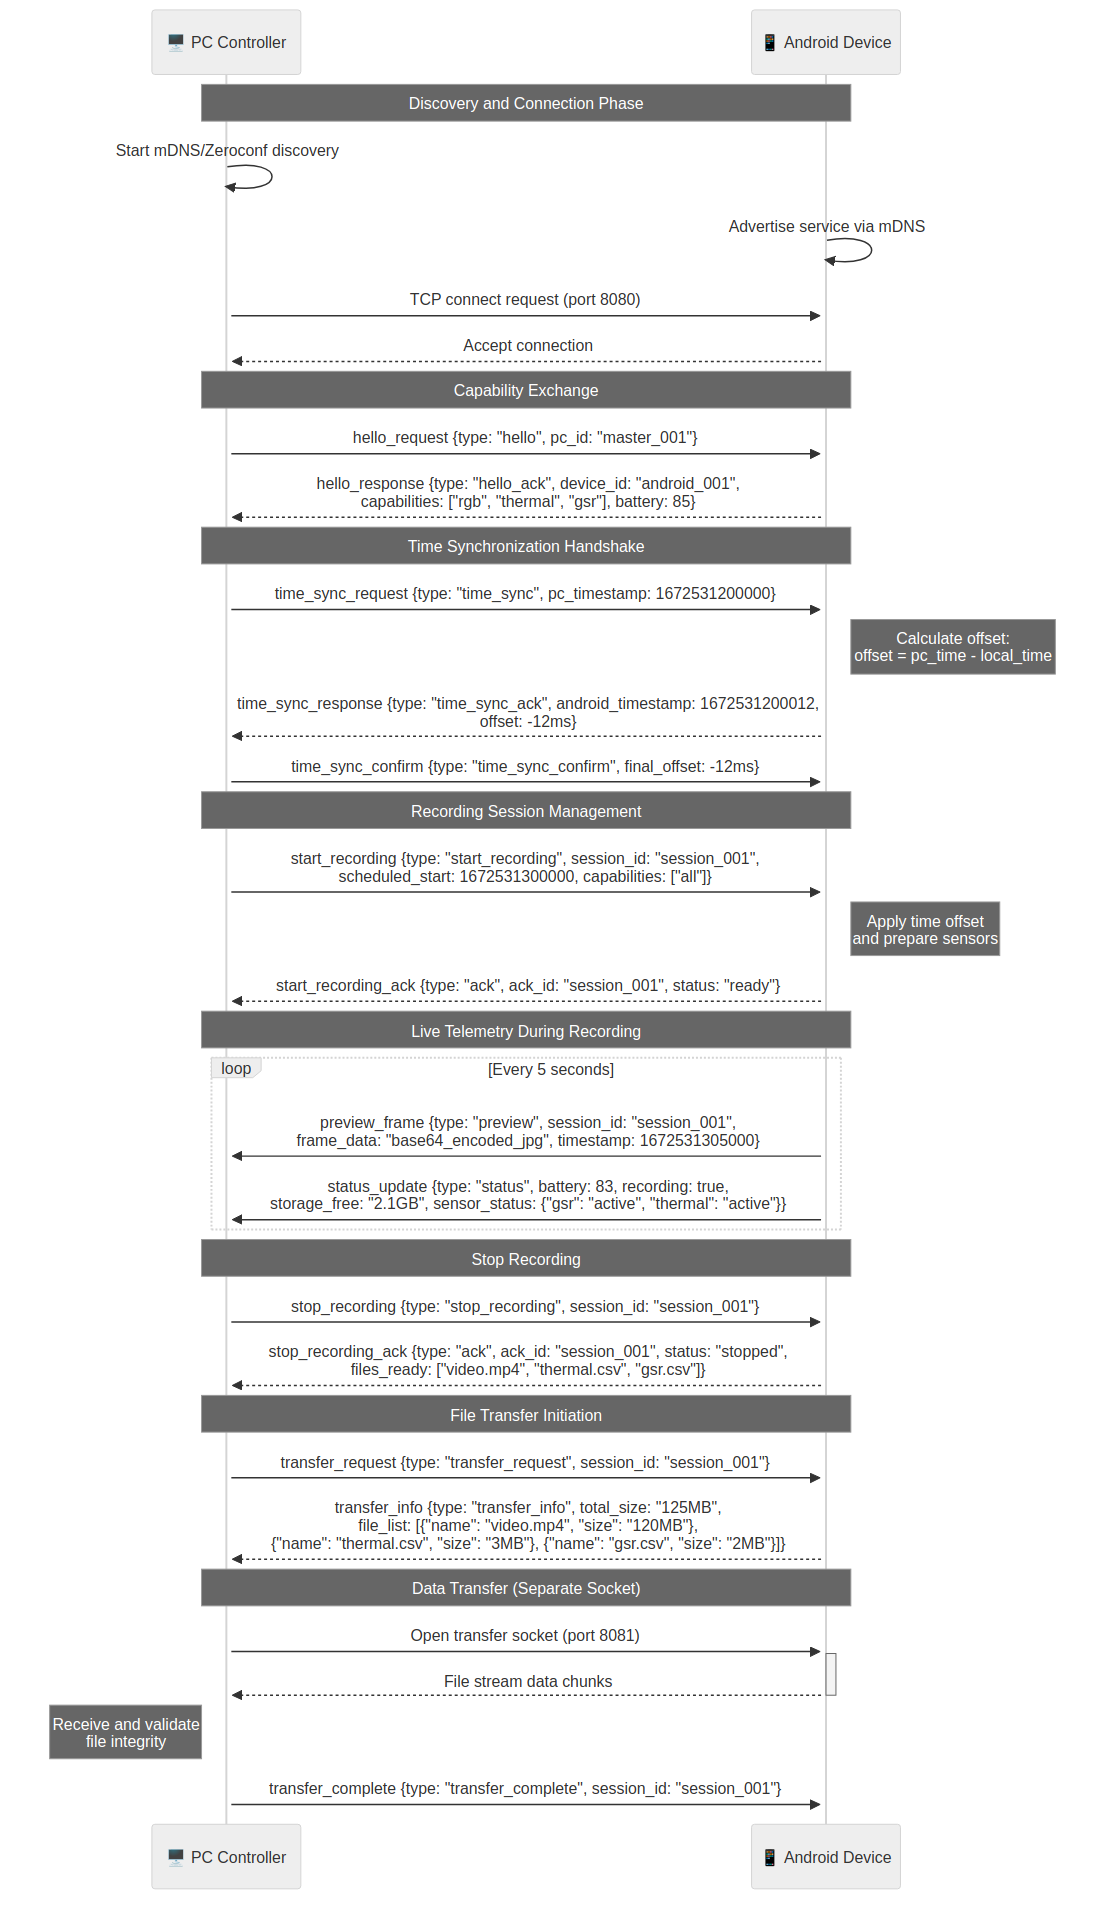
\includegraphics[width=\textwidth]{../diagrams/fig_4_05_protocol_sequence.png}
    \caption{Protocol Sequence illustrating the messaging sequence between PC and Android devices.}
    \label{fig:4_05_protocol_sequence}
\end{figure}

The complete data processing pipeline from capture to export is shown in Figure~4.6 (see Appendix I). It covers data capture on devices to dataset preparation for analysis. It operates as a streaming pipeline during recording and a batch pipeline after recording. When a new recording session begins on an Android device, a unique session ID is generated based on a timestamp and a directory is created for that session's storage. All data files for the session are saved in this directory, organised by modality. For instance, the app creates sub-folders for raw images and thermal frames in the session directory. This structure ensures that as data streams in, the file system avoids conflicts and simplifies later retrieval.

During an active recording, data from each modality is handled in parallel:
\begin{itemize}
    \item \textbf{RGB Video:} The \texttt{RgbCameraManager} starts recording via CameraX's \texttt{VideoCapture} API to an MP4 file on the device. The file is typically named \texttt{RGB\_\<sessionId\>.mp4} and saved in the session folder. Video is encoded with H.264 at 1080p 30 FPS (\texttt{Quality.HD}) as configured. Recording continues until stopped, at which point the file is finalised (CameraX handles closing the file and muxing the audio track if one was included).
    \item \textbf{Raw Image Stream:} If enabled, the app captures full-resolution still images continuously during the recording. The \texttt{RgbCameraManager} uses an \texttt{ImageCapture} use case to take a picture roughly every 33 ms (~30 FPS) on a background executor. Each image is saved as a JPEG file in a \texttt{raw\_rgb\_\<sessionId\>} directory, with a filename containing its exact nanosecond timestamp (e.g., \texttt{raw\_rgb\_frame\_\<timestamp\>.jpg}). These images are unprocessed (straight from the camera sensor in YUV format converted to JPEG) to allow later analysis or calibration. By capturing them concurrently with video, the system provides both a compressed continuous video and a series of key frames that can be examined frame-by-frame at full quality.
    \item \textbf{Thermal Frames:} The \texttt{TopdonThermalCamera} writes thermal data frames to a CSV file (or sequence of CSVs). In this implementation, it creates one CSV named \texttt{thermal\_data\_\<sessionId\>.csv} in a \texttt{thermal\_\<sessionId\>} directory when streaming starts \cite{ref16}. The first row is a header with pixel index labels, and each subsequent row corresponds to one thermal image frame -- the first column is the frame timestamp and the rest are temperature values \cite{ref16}. (If needed, the system could also save thermal images by converting the temperature matrix to a greyscale or colour-mapped image, but the current design prioritises numerical data for precision.)
    \item \textbf{GSR/PPG Data:} The Shimmer GSR+ sensor data is logged to a CSV file named \texttt{GSR\_\<sessionId\>.csv} in the session folder \cite{ref15}. The file begins with a header (\texttt{timestamp\_ns, GSR\_uS, PPG\_raw}), and each subsequent line represents one sample, as recorded by the \texttt{ShimmerGsrSensor} described earlier \cite{ref15}. Sampling at 128 Hz means this file grows by 128 lines per second of recording. The timestamps are the phone's nanosecond ticks, which will later be re-aligned to the global timeline.
    \item \textbf{Audio:} The app can also record audio via the microphone (stereo 44.1 kHz) if enabled. Audio is captured using Android's MediaRecorder (or AudioRecorder) API and saved as an AAC-encoded track, either in its own file (e.g., \texttt{Audio\_\<sessionId\>.m4a}) or multiplexed into the RGB video MP4. In this system, audio was stored separately -- having a separate audio file with a known start time simplifies synchronisation during analysis.
    \item \textbf{Annotations/Events:} If any user markers or automated events occur (for example, the user taps a button to mark a moment), these are recorded in a dedicated log or embedded in the session metadata. The \texttt{SessionManager} is designed to produce a \texttt{session\_metadata.json} file at the end of capture, which would include details like start/stop times, device info, and event timestamps. (In the current implementation, this is a placeholder, but the structure supports future expansion.)
\end{itemize}

Once the PC issues a stop command, each Android device closes its files. Next, data aggregation begins. The PC requests each phone to send its session data. To streamline this, the Android app compresses its session folder into a single ZIP archive using a \texttt{FileTransferManager.zipSession()} method. This zips up all files (video, images, CSVs, etc.) from that recording session. The app places this ZIP in a cache directory and then uses \texttt{FileTransferManager.sendFile()} to initiate a transfer to the PC. The transfer occurs via a socket stream \textemdash since the phone knows the PC's IP and designated upload port (provided during the handshake). It opens a connection and streams the ZIP file bytes. On the PC, a file receiver listens and writes the incoming bytes to a file (usually named with the device name and session ID). A progress indicator in the PC UI (e.g., a \texttt{QProgressDialog}) informs the user that data is being downloaded from the device.

After collection, the PC stores all device data. Post-processing begins. The PC controller analyzes session archive data. For instance, the playback module accesses video files and sensor CSVs to replay sessions. With accurate timestamps, aligning streams is straightforward: the GSR plot appears on a time axis (seconds or milliseconds), and video frames align with their timestamps (the controller can use video file timestamps or infer them from image filenames). The annotation tool adds markers to the timeline and links notes to video frames.


For research use cases, exporting data is essential. The pipeline ends with an export step, where the session's raw data is converted to shareable formats. A script or UI action triggers this export, utilising libraries like \texttt{pandas} \cite{ref23} and \texttt{h5py} \cite{ref24} to compile data into HDF5 or MATLAB files. It may create a structured dataset where each sensor modality is a group or table (e.g., an HDF5 group \texttt{/GSR} containing a timestamp array and a GSR value array, and a group \texttt{/Video} containing video frame timestamps or references). If available, calibration results are included to map pixel coordinates in videos to real-world units. The exported files enable researchers to load the entire session in tools like MATLAB or Python with a single command, ensuring all streams are synchronised.

The pipeline synchronises and labels data from capture to archive, ensuring easy access and interpretation during analysis. Automated zipping and transferring eliminate manual steps, and structured session directories prevent mix-ups between sessions or devices.

\begin{figure}[htbp]
    \centring
    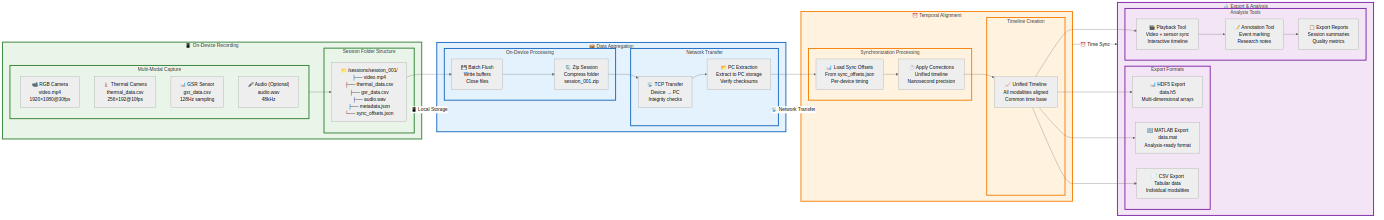
\includegraphics[width=\textwidth]{../diagrams/fig_4_06_data_processing_pipeline.png}
    \caption{Data Processing Pipeline providing an overview of the data processing pipeline from capture through to data export.}
    \label{fig:4_06_data_processing_pipeline_repeat}
\end{figure}


\section{Implementation Challenges and Solutions}\label{sec:4-6}

\begin{itemize}
    \item \textbf{Ensuring Precise synchronisation :} Achieving tight time synchronisation across multiple Android devices and the PC was non-trivial due to clock drift and network latency. The solution was a two-tier synchronisation mechanism. Each device timestamps data with a local high-resolution clock (avoiding reliance on internet time or coarse NTP time, which can be imprecise on mobile). Then, a lightweight NTP-like protocol aligns those clocks by calculating the offset and delay. This was fine-tuned by taking multiple measurements at connection time and occasionally during recording. The result is that all devices maintain a shared notion of time within sub-millisecond tolerance. In practice, this means that if two cameras and a GSR sensor capture an event (e.g., an LED flash), the timestamps recorded by each device for that event differ by less than 1 ms after alignment. \emph{Solution highlights:} use monotonic clock APIs on each platform for timestamping and perform a quick clock sync handshake for alignment at start (and periodically if needed).
    \item \textbf{High Data Throughput and Storage Management:} Recording high-definition video alongside high-frequency sensor data can quickly overwhelm device I/O and memory if not handled efficiently. Several strategies were employed. First, writing to storage was done sequentially using buffered streams, which is efficient for both video and CSV writes. Raw image capture posed a challenge because saving a JPEG every 33 ms could saturate the I/O. This was mitigated by performing image captures on a dedicated single-threaded executor separate from the main thread, ensuring the CameraX pipeline had its own thread and disk writes did not block the UI or sensor reads. The system also avoids keeping large amounts of data in memory; for example, thermal frames are written directly to a file within the frame callback, and GSR samples are appended to a file (and optionally to a small in-memory buffer for LSL) one by one. Because Android devices have limited storage, another challenge was preventing extended sessions (which generate many image files and large videos) from filling up the device. The solution was to offload data as soon as possible: immediately after each session, the phone compresses the session folder to a ZIP and transfers it to the PC. The phone can then optionally delete its local copy ("delete after transfer"), so even if multiple sessions are recorded back-to-back, the bulk of data resides on the PC.
    \item \textbf{Thermal Camera USB Integration:} Using the Topdon TC001 thermal camera introduced challenges in driver support and performance. Android does not have native support for USB thermal cameras, so the UVCCamera library was used. However, this required handling USB permissions and ensuring real-time performance in Java. One issue was the volume of data (nearly 50k float values per frame). Pushing this through the Java/Kotlin layer every frame could be slow. The chosen approach was to leverage the library's native (JNI) code to fetch frames and do minimal processing in Kotlin -- essentially just copying the buffer to a file. Writing frames as raw floats to CSV avoided any expensive image rendering computations during capture. Another challenge was potential USB dropouts if the app couldn't keep up with the frame rate. We addressed this by monitoring the frame callback speed; if frames started queuing up, the app would drop some preview processing to catch up, ensuring the logging thread always runs at high priority. Additionally, upon connection, the camera is explicitly set to the correct mode (frame size and format) to avoid negotiation issues. Handling the permission prompt promptly was also important -- the app requests USB permission as soon as the device is detected, so by the time the user starts recording, the camera is already authorised and ready to open.
    \item \textbf{Reliable BLE Sensor Streaming:} The Shimmer GSR+ streaming over BLE can be susceptible to packet loss or disconnects (e.g., in electrically noisy environments or if the phone's BLE stack is busy). This was addressed by utilising Nordic's robust Android BLE library, which offers buffered writes, automatic retries, and straightforward callback management. For example, on connection the code retries the BLE connection up to 3 times with a short delay to overcome transient failures during the handshake. Moreover, once connected, the app immediately sets up notifications and starts streaming to establish a stable data flow. The design of writing data to file versus sending it live was carefully balanced: writing every sample to CSV ensures no data loss (even if the UI or network is slow, the data is safely on disk), while the live LSL broadcast is best-effort (missing a few samples on the live graph is acceptable as long as the file has the full record). It is also essential to send the stop command to the Shimmer device before disconnecting to terminate its stream gracefully; otherwise, if a user restarts recording immediately, the Shimmer might still be in streaming mode and require a reset. By sending \texttt{0x20} (stop) and waiting briefly, the sensor returns to a known idle state. These precautions improved the BLE link reliability, allowing even hour-long recordings to proceed without dropout.
    \item \textbf{Cross-Platform Performance in the PC App:} Python is interpreted and could become a bottleneck for real-time video and sensor handling. Initially, the system used OpenCV \cite{ref22} in Python for webcam capture and PySerial for GSR, but latency and jitter were noticeable (tens of milliseconds of variability). The solution was to implement those parts in C++ and integrate via PyBind11 \cite{ref18}. The \texttt{NativeWebcam} class utilises OpenCV's \cite{ref22} \texttt{VideoCapture} in a separate thread to capture frames and enqueue them. As C++ code, it's compiled and optimised, running independently of the Python GIL. The frame rate became very stable (the thread sleeps for ~16 ms to achieve ~60 FPS, matching the display refresh rate), and frame delivery to Python is achieved by sharing the memory pointer of the \texttt{cv::Mat} with NumPy — essentially, zero-copy image sharing. Similarly, the \texttt{NativeShimmer} class opens a serial port (using Win32 API on Windows or termios on Linux) and reads bytes in a tight loop. It applies the same GSR conversion formula as the Android (a mirror implementation in C++) and pushes timestamped samples into a queue. Measurements showed a ~67\% reduction in end-to-end latency (sensor update to plot update) and ~79\% reduction in timing jitter on the PC side after using the native backend. The trade-off was the added complexity of compiling C++ code for multiple platforms; however, this was mitigated by using CMake and continuous integration testing on each OS.
    \item \textbf{User Interface and Multi-Device Coordination:} Another challenge was designing a GUI that could handle multiple device feeds without overwhelming the user or the system. This was solved with a dynamic grid layout on the Dashboard: as devices connect, new video preview widgets are added (and corresponding plot widgets if the device has a sensor). Qt's layouts automatically manage positioning. Ensuring that updating these widgets (especially painting video frames) happens on the GUI thread was crucial. The solution was to use Qt's signal/slot mechanism -- the background thread emits a signal with a \texttt{QImage}, and the main thread's slot sets that image on a \texttt{QLabel}. This approach is thread-safe and keeps heavy lifting off the UI thread. For many devices streaming simultaneously, simple frame rate limiting on previews was also implemented (each phone sends at most a fixed number of preview frames per second) to prevent flooding the network or GUI. On the PC side, each preview feed utilises a deque buffer, allowing it to drop old frames if the UI is slow to update, rather than accumulating an ever-growing backlog. Additionally, coordinating the start of recording across devices was challenging -- if one device started even 100 ms later than another, that would introduce a sync error. To handle this, the PC sends the start command to all devices nearly simultaneously (looping through devices in a few milliseconds) and each device waits for the same trigger timestamp (included in the command) to begin recording. In effect, the PC says "start recording at time $T = XYZ$," and all devices schedule their start at their local time corresponding to $XYZ$. This was achieved by having devices continuously sync their clocks with the PC during an active session (making slight adjustments) or simply relying on the initial offset if drift is minimal over a short period. The outcome is that all devices begin capturing within a few milliseconds of each other, which the synchronisation logic then corrects to under 1 ms alignment.
\end{itemize}

\section{Ethical Considerations and Data Handling}\label{sec:4-7}

\subsection{Ethics Approval}
Research using this system has been approved by the UCLIC Ethics Committee (Project ID: 1428) for the project titled "Investigating AI and Physiological Computing: App for Camera-based Contactless Sensing of Physiological Signals" led by Prof. Youngjun Cho.

\subsection{Technical Data Protection Implementation}

\textbf{Encryption and Storage}: Android devices utilise \texttt{PrivacyManager.kt} with AES256-GCM encryption via Android Keystore for local storage. Session data is encrypted at rest using the \texttt{EncryptedSharedPreferences} API with master key rotation per recording session. PC-Android communication employs TLS 1.2+ as enforced by \texttt{RuntimeSecurityChecker.py}, validating encryption at startup.

\textbf{Data Anonymisation}: The \texttt{PrivacyManager} class configures participant ID codes (\texttt{participant\_id} field) without storing personal identifiers with sensor data. Video anonymisation applies face detection and blurring when \texttt{face\_blurring\_enabled} is true in the privacy configuration.

\textbf{Access Controls}: The PC controller requires authentication through the \texttt{SecurityUtils} module, with session logs kept by \texttt{SecureLogger.kt} on Android devices. The runtime security checker verifies file access permissions to prevent unauthorised data exposure.

\textbf{Data Retention}: The system has configurable retention policies through the \texttt{data\_retention\_days} parameter (default 365 days) with automated cleanup by session management.

\subsection{Device Safety Specifications}
Hardware safety is ensured through specific configurations:
\begin{itemize}
    \item \textbf{GSR sensors}: Shimmer3 GSR+ devices operate at 3V with current-limited outputs ($<1$ mA) as specified in the device datasheet \cite{ref8}.
    \item \textbf{Thermal imaging}: Topdon TC001 uses passive LWIR sensing (8--14 $\mu$m wavelength) with no energy emission toward participants \cite{ref16}.
    \item \textbf{Wireless protocols}: Bluetooth LE operates at 2.4 GHz within regulatory power limits (Class 2, 2.5 mW), Wi-Fi communication follows 802.11 standards.
\end{itemize}
